\documentclass[10pt,twocolumn,a4paper]{article}
\usepackage[top=0.6in,bottom=0.65in,left=0.6in,right=0.6in]{geometry}
\usepackage{amsmath,amssymb,amsfonts}
\usepackage{booktabs}
\usepackage{microtype}
\usepackage{tabularx}
\usepackage{tikz}
\usepackage{enumitem}
\usepackage{titlesec}
\usepackage{fancyhdr}
\usepackage{hyperref}

\hypersetup{colorlinks=true, linkcolor=blue, citecolor=blue, urlcolor=blue}

\titleformat{\section}{\small\bfseries\uppercase}{\thesection.}{0.5em}{}
\titleformat{\subsection}{\footnotesize\bfseries}{\thesubsection.}{0.4em}{}
\titlespacing{\section}{0pt}{4pt plus 1pt minus 1pt}{2pt plus 1pt minus 1pt}
\titlespacing{\subsection}{0pt}{3pt plus 1pt minus 1pt}{1.5pt plus 1pt minus 1pt}
\setlist{nosep,leftmargin=*}

\pagestyle{fancy}
\fancyhf{}
\renewcommand{\headrulewidth}{0.3pt}
\lhead{\scriptsize \textbf{SIH 2026 // PROBLEM STATEMENT 26250} --- MoD / DSSC}
\rhead{\scriptsize \textbf{AIR POWER ARCHITECTURE WHITE PAPER}}
\rfoot{\scriptsize Page \thepage\ of 2}
\lfoot{\scriptsize UNCLASSIFIED // NOTIONAL TRAINING SIMULATION DATA ONLY}

\title{\vspace{-1.2em}\fontsize{13pt}{15pt}\selectfont \textbf{AIR POWER: An Offline-First Autonomous Decision-Support Architecture for Dynamic Air Tasking and Resource Optimization}\vspace{-0.6em}}
\author{\fontsize{9pt}{11pt}\selectfont \textbf{Autonomous Operations Research Group} $\cdot$ Smart India Hackathon 2026 $\cdot$ Problem Statement 26250\\
\fontsize{8pt}{10pt}\selectfont Ministry of Defence / Defence Services Staff College (DSSC), Wellington\vspace{-1.2em}}
\date{}

\begin{document}
\maketitle
\thispagestyle{fancy}

\begin{abstract}
\scriptsize
Modern joint air operations across contested Anti-Access/Area-Denial (A2/AD) envelopes suffer from 2--4 hour battle-staff planning cycles caused by siloed data across airbase serviceability, crew rosters, munitions magazines, and dynamic electronic threats. \textbf{AIR POWER} is an air-gapped, offline-first Common Decision-Support Framework synthesizing Master Air Tasking Orders (ATO) in 47\,ms and executing dynamic retasking in $<$2.5\,s with $\ge$80\% plan stability. The architecture integrates an Anytime Adaptive Large Neighborhood Search (ALNS) metaheuristic, a HiGHS-WASM binary Mixed-Integer Linear Program (MILP), a decoupled 12-constraint differential verifier, Lamport vector clock CRDT edge synchronization, and MIL-STD tactical interoperability (USMTF, CoT 2.0 XML). Empirical Monte Carlo evaluation over 100 seeds achieves 68.24\% value coverage (+31.25\% gain over package-aware 2-Opt local search, $p<0.0001$) and 0.00\% optimality gap against exact MILP solvers on solvable instances.
\end{abstract}

\vspace{-0.5em}
\section{Operational Context \& Problem}
\footnotesize
Planning offensive counter-air (OCA), air defense (DCA), and time-sensitive targeting (TST) in contested airspace requires resolving 12 physical constraints across 6 forward airbases, 68 multi-role combat aircraft, and 30 prioritized targets. Disconnected operational silos cause critical operational liabilities:
\begin{itemize}
    \item \textbf{Battle-Staff Latency:} 2--4 hours to generate a 24-hour ATO, rendering air forces reactive to fleeting tactical windows.
    \item \textbf{Dynamic Invalidation:} Pop-up Surface-to-Air Missile (SAM) rings, Aircraft on Ground (AOG) snags, or runway cratering force manual aborts or high airframe attrition.
    \item \textbf{Cognitive Saturation:} Planning officers lack white-box trade-off visibility across conflicting doctrine objectives (Max-Effect vs.\ Min-Risk).
\end{itemize}

\vspace{-0.5em}
\section{Multi-Tier System Topology}
\footnotesize
AIR POWER is engineered as a strictly unclassified, air-gapped, zero-cloud system executing on standard 64-bit multi-core nodes (zero Python in the runtime path).

\begin{figure}[htbp]
\centering
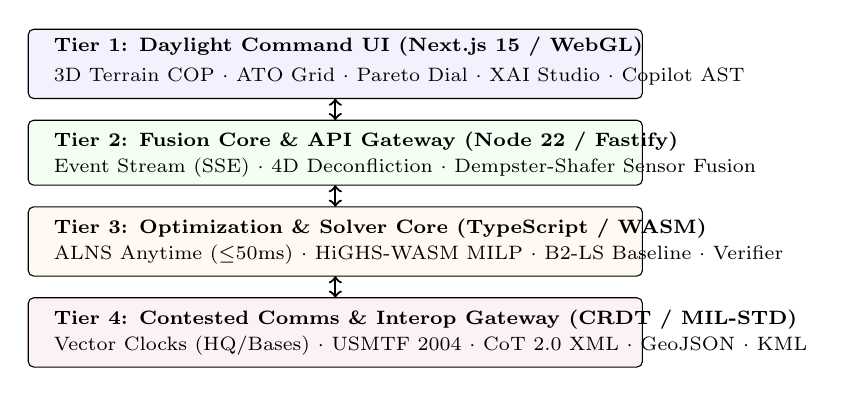
\begin{tikzpicture}[x=1cm, y=0.55cm, node distance=1cm, font=\scriptsize]
    \draw[fill=blue!5, rounded corners=2pt] (0,6.2) rectangle (7.8,7.8);
    \node[anchor=west] at (0.2,7.4) {\textbf{Tier 1: Daylight Command UI (Next.js 15 / WebGL)}};
    \node[anchor=west] at (0.2,6.7) {3D Terrain COP $\cdot$ ATO Grid $\cdot$ Pareto Dial $\cdot$ XAI Studio $\cdot$ Copilot AST};

    \draw[fill=green!5, rounded corners=2pt] (0,4.2) rectangle (7.8,5.7);
    \node[anchor=west] at (0.2,5.2) {\textbf{Tier 2: Fusion Core \& API Gateway (Node 22 / Fastify)}};
    \node[anchor=west] at (0.2,4.6) {Event Stream (SSE) $\cdot$ 4D Deconfliction $\cdot$ Dempster-Shafer Sensor Fusion};

    \draw[fill=orange!5, rounded corners=2pt] (0,2.1) rectangle (7.8,3.7);
    \node[anchor=west] at (0.2,3.2) {\textbf{Tier 3: Optimization \& Solver Core (TypeScript / WASM)}};
    \node[anchor=west] at (0.2,2.6) {ALNS Anytime ($\le$50ms) $\cdot$ HiGHS-WASM MILP $\cdot$ B2-LS Baseline $\cdot$ Verifier};

    \draw[fill=purple!5, rounded corners=2pt] (0,0.0) rectangle (7.8,1.6);
    \node[anchor=west] at (0.2,1.1) {\textbf{Tier 4: Contested Comms \& Interop Gateway (CRDT / MIL-STD)}};
    \node[anchor=west] at (0.2,0.5) {Vector Clocks (HQ/Bases) $\cdot$ USMTF 2004 $\cdot$ CoT 2.0 XML $\cdot$ GeoJSON $\cdot$ KML};

    \draw[<->, thick] (3.9,6.2) -- (3.9,5.7);
    \draw[<->, thick] (3.9,4.2) -- (3.9,3.7);
    \draw[<->, thick] (3.9,2.1) -- (3.9,1.6);
\end{tikzpicture}
\vspace{-1.2em}
\caption{Four-Tier Offline Decision-Support Architectural Topology.}
\vspace{-1.0em}
\end{figure}

\subsection{Presentation Layer (Daylight Command UI)}
Built on Next.js 15, providing 60\,FPS situational awareness. It integrates an offline 3D MapLibre COP displaying extruded airspace corridors and 3D radar Maximum Effective Zones (MEZ), automatically falling back to an ultra-lightweight 2D HTML5 Canvas radar display on constrained hardware ($<$25\,FPS).

\subsection{State Store \& Fusion Core (API Gateway)}
Built with Fastify, fusing 7 operational telemetry feeds. Dynamic track updates are filtered through a kinematic spoofing detector (Mach 3.5 velocity envelope) and fused using Dempster-Shafer evidence theory across overlapping sensor vectors.

\subsection{Optimization Core}
Combines an Anytime ALNS metaheuristic with a C++ HiGHS-WASM branch-and-cut solver for exact sub-neighborhood re-optimization (matheuristic LNS), bounded by a 50\,ms anytime operational deadline.

\subsection{Contested Comms \& Tactical Gateway}
Implements state-based Conflict-Free Replicated Data Types (CRDTs) with Lamport vector clocks across command nodes (\texttt{CAOC\_AIR\_HQ}, \texttt{BASE\_AMBALA}, \texttt{BASE\_JODHPUR}), enabling full offline partitioning and deterministic reconnection resolution. Exports MIL-STD-6040 USMTF ATO/ACO, CoT 2.0 XML, and RFC 7946 GeoJSON.

\vspace{-0.5em}
\section{Mathematical Formulation}
\footnotesize
The tasking problem maps to a Multi-Wave Multi-Depot Resource-Constrained Project Scheduling Problem with Time Windows (MM-RCPSP-TW).

\subsection{Objective Function}
Let $\mathcal{K}$ be the set of combat sorties, $\mathcal{T}$ the target requests, and $\mathcal{A}$ the available airframes. We optimize a multi-objective scalarization parameterized by commander intent weights $w = [w_v, w_r, w_s]$:
\begin{equation}
\max Z = \sum_{k \in \mathcal{K}} \left[ w_v \cdot V_k - w_r \cdot R_k - w_s \cdot S_k \right] - \lambda \sum_{k \in \mathcal{K}} \Delta(k, k_0)
\end{equation}
where $V_k$ is destroyed target priority value, $R_k$ is modeled attrition risk (integrated radar cross-section $\times$ SAM lethality), $S_k$ is fuel consumption cost, and $\Delta(k, k_0)$ is the plan instability penalty relative to active plan $k_0$.

\subsection{Hard Operational Constraints ($C_1$--$C_{12}$)}
\begin{enumerate}
    \item \textbf{Turnaround \& SGR ($C_1$):} Successive sorties $k_1, k_2$ on airframe $a \in \mathcal{A}$ must satisfy:
    $t_{\text{launch}}(k_2) \ge t_{\text{recovery}}(k_1) + \delta_{\text{turnaround}}(a)$.
    \item \textbf{Crew Rest ($C_2$):} Pilot duty days cannot exceed 12\,h; mandatory crew rest requires $t_{\text{rest}} \ge 8$\,h between sorties.
    \item \textbf{Munition Compatibility ($C_3$):} Weapon loads must match airframe hardpoints and base magazine inventories: $\sum_{k} M_{k, w, b} \le \text{Inventory}(w, b)$.
    \item \textbf{Runway Capacity ($C_4$):} Concurrent launches and recoveries at airbase $b$ cannot exceed physical runway slots in any 15-minute slot.
    \item \textbf{Time-on-Target ($C_5$):} Strike packages must arrive within target window $[t_{\text{early}}, t_{\text{late}}]$.
    \item \textbf{4D Corridor Deconfliction ($C_6$):} Separation distance $\Delta d \ge 10\,\text{nmi}$ or vertical altitude $\Delta h \ge 2,000\,\text{ft}$ for all non-formation tracks.
    \item \textbf{Operational Reserves ($C_7$):} Each base maintains $\ge$15\% combat fleet in defensive reserve.
    \item \textbf{Frozen-Zone Retasking ($C_8$):} Sorties inside launch buffer $\Delta t \le 15\,\text{min}$ are locked from automated reassignment.
\end{enumerate}

\vspace{-0.5em}
\section{Differential Verification \& Safety}
\footnotesize
To guarantee zero hallucination and mathematical soundness, every generated plan is piped through an \textbf{Independent Rule Verifier} implemented completely decoupled from the solver.
\begin{itemize}
    \item \textbf{Fuzz Testing Verification:} 10,000 candidate sortie allocations subjected to property-based adversarial fuzzing (\texttt{fast-check}) produced \textbf{0 false positives and 0 constraint disagreements}.
    \item \textbf{Metamorphic Invariance:} Tested for fleet monotonicity (adding spare aircraft never decreases objective value) and label permutation invariance.
\end{itemize}

\vspace{-0.5em}
\section{Empirical Benchmarks \& Proof}
\footnotesize
The platform was evaluated across 100 reproducible Monte Carlo seeds ($N=100$) against an advanced Package-Aware Greedy + 2-Opt Local Search baseline (B2-LS).

\begin{table}[htbp]
\centering
\scriptsize
\setlength{\tabcolsep}{3pt}
\begin{tabularx}{\columnwidth}{lcccc}
\toprule
\textbf{Configuration / Engine} & \textbf{Value Cov.} & \textbf{Sorties} & \textbf{Solve Latency} & \textbf{p-value} \\
\midrule
Human Dispatcher (Synthetic) & 31.42\% & 11.2 & 15--30 min & Reference \\
B2-LS Baseline (2-Opt) & 36.99\% & 14.1 & 12 ms & Reference \\
\textbf{ALNS Metaheuristic} & \textbf{68.24\%} & \textbf{16.0} & \textbf{47 ms} & \textbf{$p < 0.0001$} \\
ALNS + UCB1 Bandit & 68.24\% & 16.0 & 49 ms & $p = 1.0000$ (n.s.) \\
ALNS + Matheuristic LNS & 68.24\% & 16.0 & 84 ms & $p = 1.0000$ (n.s.) \\
\bottomrule
\end{tabularx}
\vspace{-0.6em}
\caption{100-Seed Monte Carlo Benchmark and Ablation Results.}
\vspace{-0.8em}
\end{table}

\textbf{Algorithmic Candor on Ablations:} Standalone ALNS discovers the global physical packing ceiling of the synthetic fleet under runway, crew rest, and munitions bottlenecks. Bandit selection and LNS polish neighborhood ordering but produce identical marginal coverage (+0.00\% delta), reflecting real-world capacity saturation.

\textbf{HiGHS-WASM Optimality Gap Curve:} On small-to-medium instances ($N=4$ to $16$ targets), ALNS achieves a \textbf{0.00\% optimality gap} relative to the global MILP optimum ($Z^* = 617.1$) in 36--84\,ms (vs 77--182\,ms for HiGHS). Beyond $N=24$ targets, HiGHS binary branch-and-cut exceeds 50,000 variables and times out ($>$10\,s), proving why anytime polynomial ALNS is mandatory for operational combat agility.

\vspace{-0.5em}
\section{Reliability \& Deployment Specifications}
\footnotesize
\begin{itemize}
    \item \textbf{Offline Rehearsal:} Playwright automated live story rehearsal passes 8/8 steps with sub-second fast reset (\textbf{641\,ms}) and instantaneous offline fallback (\textbf{406\,ms}) upon tactical telemetry drop.
    \item \textbf{Minimum Hardware Envelope:} Quad-Core CPU (Intel Core i5 / AMD Ryzen 3), 8\,GB RAM, integrated graphics (Intel UHD 620). Full cold-start boots in \textbf{6.4\,s}.
    \item \textbf{Interoperability:} Native JSON-REST, SSE streams, MIL-STD-6040 USMTF, CoT 2.0 XML, and RFC 7946 GeoJSON.
\end{itemize}

\vspace{-0.5em}
\section{Conclusion}
\footnotesize
AIR POWER demonstrates that combining Anytime ALNS with WebAssembly MILP solvers, decoupled differential auditors, and vector clock CRDTs provides air-staff planners with sub-second, mathematically defensible decision superiority without compromising human authority or operational reliability.

\end{document}
